\documentclass{beamer}
\usepackage[utf8]{inputenc}

\usetheme{Madrid}
\usecolortheme{default}
\usepackage{amsmath,amssymb,amsfonts,amsthm}
\usepackage{txfonts}
\usepackage{tkz-euclide}
\usepackage{listings}
\usepackage{adjustbox}
\usepackage{array}
\usepackage{tabularx}
\usepackage{gvv}
\usepackage{lmodern}
\usepackage{circuitikz}
\usepackage{tikz}
\usepackage{graphicx}

\setbeamertemplate{page number in head/foot}[totalframenumber]

\usepackage{tcolorbox}
\tcbuselibrary{minted,breakable,xparse,skins}



\definecolor{bg}{gray}{0.95}
\DeclareTCBListing{mintedbox}{O{}m!O{}}{%
	breakable=true,
	listing engine=minted,
	listing only,
	minted language=#2,
	minted style=default,
	minted options={%
		linenos,
		gobble=0,
		breaklines=true,
		breakafter=,,
		fontsize=\small,
		numbersep=8pt,
		#1},
	boxsep=0pt,
	left skip=0pt,
	right skip=0pt,
	left=25pt,
	right=0pt,
	top=3pt,
	bottom=3pt,
	arc=5pt,
	leftrule=0pt,
	rightrule=0pt,
	bottomrule=2pt,
	toprule=2pt,
	colback=bg,
	colframe=orange!70,
	enhanced,
	overlay={%
		\begin{tcbclipinterior}
			\fill[orange!20!white] (frame.south west) rectangle ([xshift=20pt]frame.north west);
	\end{tcbclipinterior}},
	#3,
}
\lstset{
	language=C,
	basicstyle=\ttfamily\small,
	keywordstyle=\color{blue},
	stringstyle=\color{orange},
	commentstyle=\color{green!60!black},
	numbers=left,
	numberstyle=\tiny\color{gray},
	breaklines=true,
	showstringspaces=false,
}
%------------------------------------------------------------
%This block of code defines the information to appear in the
%Title page
\title %optional
{4.7.34}
\date{}
%\subtitle{A short story}

\author % (optional)
{M Chanakya Srinivas- EE25BTECH11036}




\begin{document}


\frame{\titlepage}


\begin{frame}{Problem Statement}
Find the equation of a plane at a distance $3\sqrt{3}$ from the origin, 
whose normal is equally inclined to the coordinate axes.
\end{frame}

\begin{frame}{Normal Vector}
If the normal is equally inclined to all coordinate axes:
\begin{align}
\vec{n} &= \lambda \myvec{1\\1\\1}, \quad \lambda \neq 0
\end{align}
\end{frame}

\begin{frame}{Equation of Plane}
The general equation of a plane is:
\begin{align}
\vec{n}^\top \vec{x} &= p
\end{align}
\end{frame}

\begin{frame}{Distance Condition}
Distance of the plane from the origin:
\begin{align}
d &= \frac{|p|}{\|\vec{n}\|} \\
\|\vec{n}\| &= |\lambda|\sqrt{1^2+1^2+1^2} = |\lambda|\sqrt{3}
\end{align}
Substitute $d = 3\sqrt{3}$:
\begin{align}
3\sqrt{3} &= \frac{|p|}{|\lambda|\sqrt{3}} \\
|p| &= 9|\lambda|
\end{align}
\end{frame}

\begin{frame}{Simplification}
Divide through by $\lambda$:
\begin{align}
\myvec{1 & 1 & 1}\vec{x} &= \frac{p}{\lambda}
\end{align}
Since $\tfrac{p}{\lambda} = \pm 9$:
\begin{align}
\myvec{1 & 1 & 1}\vec{x} &= 9 \\
\myvec{1 & 1 & 1}\vec{x} &= -9
\end{align}
\end{frame}

\begin{frame}{Final Answer}
\textbf{Vector Form:}
\begin{align}
\vec{n}^\top \vec{x} &= \pm 9, \quad 
\vec{n} = \myvec{1\\1\\1}
\end{align}

\textbf{Algebraic Form:}
\begin{align}
x+y+z &= 9 \\
x+y+z &= -9
\end{align}
\end{frame}



\begin{frame}[fragile]{C CODE}
\begin{lstlisting}
#include <math.h>

void equal_inclined_planes(double distance, double *coeffs_out)
{
    if (!coeffs_out) return;
    if (distance < 0) distance = -distance;

    double a = 1.0, b = 1.0, c = 1.0;
    double rhs = distance * sqrt(3.0);

    coeffs_out[0] = a; coeffs_out[1] = b; coeffs_out[2] = c; coeffs_out[3] =  rhs;
    coeffs_out[4] = a; coeffs_out[5] = b; coeffs_out[6] = c; coeffs_out[7] = -rhs;
}
 \end{lstlisting}
\end{frame}

\begin{frame}[fragile]{Python code through shared output}
\begin{lstlisting}
# call_planes.py
from ctypes import CDLL, c_double
import math
import numpy as np
import matplotlib.pyplot as plt

# Load library
lib = CDLL('./libplanes.so')
lib.equal_inclined_planes.argtypes = (c_double, c_double * 8)
lib.equal_inclined_planes.restype = None

# Prepare output array
coeffs = (c_double * 8)()
distance = 3.0 * math.sqrt(3.0)
 \end{lstlisting}
\end{frame}
\begin{frame}[fragile]{Python code through shared output}
\begin{lstlisting}
# Call C function
lib.equal_inclined_planes(distance, coeffs)

# Extract coefficients
a1,b1,c1,d1 = coeffs[0], coeffs[1], coeffs[2], coeffs[3]
a2,b2,c2,d2 = coeffs[4], coeffs[5], coeffs[6], coeffs[7]

print(f"Plane 1: {a1}x + {b1}y + {c1}z = {d1}")
print(f"Plane 2: {a2}x + {b2}y + {c2}z = {d2}")

# -------------------
# Plotting
# -------------------
fig = plt.figure()
ax = fig.add_subplot(111, projection='3d')

# Grid for plotting planes
xx, yy = np.meshgrid(np.linspace(-10,10,20), np.linspace(-10,10,20))
 \end{lstlisting}
\end{frame}
\begin{frame}[fragile]{Python code through shared output}
\begin{lstlisting}
# Plane 1: z = (d1 - a1*xx - b1*yy)/c1
zz1 = (d1 - a1*xx - b1*yy)/c1
ax.plot_surface(xx, yy, zz1, alpha=0.3, color='cyan')

# Plane 2: z = (d2 - a2*xx - b2*yy)/c2
zz2 = (d2 - a2*xx - b2*yy)/c2
ax.plot_surface(xx, yy, zz2, alpha=0.3, color='magenta')

# Origin
ax.scatter(0,0,0, color='black', s=60, label="Origin")

ax.set_xlabel("X")
ax.set_ylabel("Y")
ax.set_zlabel("Z")
ax.legend()
plt.show()
 \end{lstlisting}
\end{frame}
\begin{frame}[fragile]{only Python code}
\begin{lstlisting}
import sys
sys.path.insert(0, '/sdcard/github/matgeo/codes/CoordGeo')  # Your custom path
import numpy as np
import matplotlib.pyplot as plt
from mpl_toolkits.mplot3d import Axes3D
# Local imports (keeping as requested)
from line.funcs import *
from triangle.funcs import *
from conics.funcs import circ_gen
# Plane coefficients: a = b = c = 1, distance from origin = 3 * sqrt(3)
a, b, c = 1, 1, 1
d1 = -9   # Plane 1: x + y + z = 9  (rewrite as x + y + z - 9 = 0)
d2 = 9    # Plane 2: x + y + z = -9 (rewrite as x + y + z + 9 = 0)
 \end{lstlisting}
\end{frame}
\begin{frame}[fragile]{only Python code}
\begin{lstlisting}
# Create grid for x and y
x = np.linspace(-10, 10, 50)
y = np.linspace(-10, 10, 50)
X, Y = np.meshgrid(x, y)
# Calculate corresponding z for both planes
Z1 = (-a * X - b * Y - d1) / c
Z2 = (-a * X - b * Y - d2) / c
# Create figure and 3D axis
fig = plt.figure(figsize=(10, 8))
ax = fig.add_subplot(111, projection='3d')
# Plot both planes with transparency and different colors
ax.plot_surface(X, Y, Z1, alpha=0.5, color='cyan', rstride=1, cstride=1, edgecolor='none', label='Plane 1: x+y+z=9')
ax.plot_surface(X, Y, Z2, alpha=0.5, color='orange', rstride=1, cstride=1, edgecolor='none', label='Plane 2: x+y+z=-9')
 \end{lstlisting}
\end{frame}
\begin{frame}[fragile]{only Python code}
\begin{lstlisting}
# Mark the origin
ax.scatter(0, 0, 0, color='red', s=80, label='Origin (0,0,0)')
# Normal vector (same for both planes)
normal_vec = np.array([a, b, c])
origin = np.array([0, 0, 0])
ax.quiver(*origin, *normal_vec, length=7, color='black', linewidth=2, label='Normal Vector (1,1,1)')
# Annotate the intercepts of Plane 1 (where x=0,y=0 -> z=9 etc)
intercepts_p1 = np.array([[9, 0, 0], [0, 9, 0], [0, 0, 9]])
for i, point in enumerate(intercepts_p1):
    ax.scatter(*point, color='blue', s=60)
    ax.text(*point, f'P{i+1}\n({point[0]}, {point[1]}, {point[2]})', color='blue', fontsize=10, ha='left')
 \end{lstlisting}
\end{frame}
\begin{frame}[fragile]{only Python code}
\begin{lstlisting}
# Annotate the intercepts of Plane 2
intercepts_p2 = np.array([[-9, 0, 0], [0, -9, 0], [0, 0, -9]])
for i, point in enumerate(intercepts_p2):
    ax.scatter(*point, color='darkorange', s=60)
    ax.text(*point, f'Q{i+1}\n({point[0]}, {point[1]}, {point[2]})', color='darkorange', fontsize=10, ha='right')
# Set labels and title
ax.set_xlabel('X-axis')
ax.set_ylabel('Y-axis')
ax.set_zlabel('Z-axis')
ax.set_title('Planes $x + y + z = 9$ and $x + y + z = -9$ with normal vector\nDistance from origin = $3\\sqrt{3}$')
# Set limits and equal aspect ratio for better view
ax.set_xlim(-12, 12)
ax.set_ylim(-12, 12)
 \end{lstlisting}
\end{frame}
\begin{frame}[fragile]{only Python code}
\begin{lstlisting}
ax.set_zlim(-12, 12)
ax.set_box_aspect([1, 1, 1])
# Add legend manually because plot_surface does not support label param well
from matplotlib.lines import Line2D
legend_elements = [
    Line2D([0], [0], color='cyan', lw=8, label='Plane 1: x + y + z = 9'),
    Line2D([0], [0], color='orange', lw=8, label='Plane 2: x + y + z = -9'),
    Line2D([0], [0], marker='o', color='w', label='Origin', markerfacecolor='red', markersize=10),
    Line2D([0], [0], color='black', lw=2, label='Normal Vector (1,1,1)'),
    Line2D([0], [0], marker='o', color='w', label='Plane 1 intercepts', markerfacecolor='blue', markersize=8),
    Line2D([0], [0], marker='o', color='w', label='Plane 2 intercepts', markerfacecolor='darkorange', markersize=8),
]
ax.legend(handles=legend_elements, loc='upper left')
plt.grid(True)
plt.show()
 \end{lstlisting}
\end{frame}
\begin{frame}[fragile]{PLOTS}
\begin{figure}
    \centering
    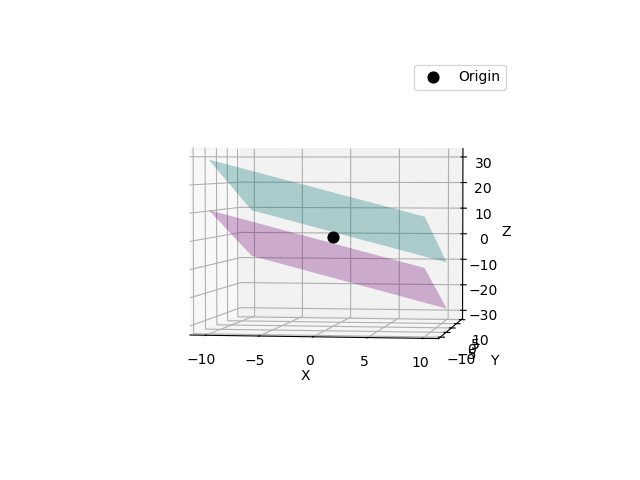
\includegraphics[width=0.9\columnwidth]{figs/fig71.png}
    \caption{}
    \label{fig:placeholder}
\end{figure}
\end{frame}
\begin{frame}[fragile]{PLOTS}
\begin{figure}
    \centering
    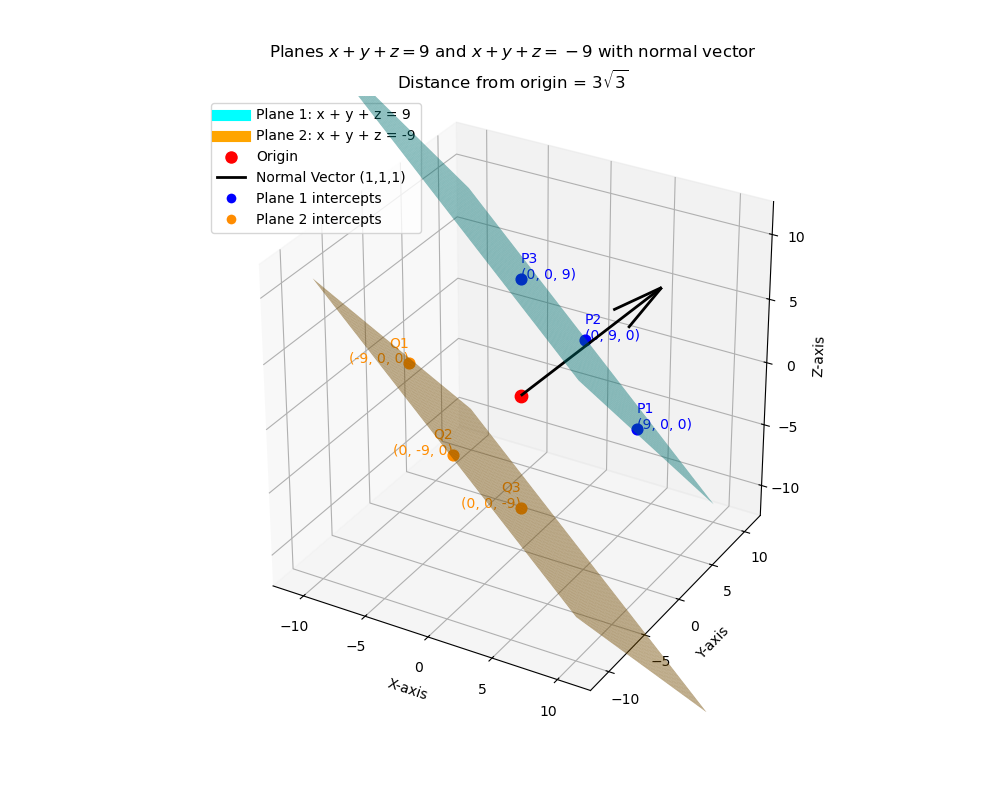
\includegraphics[width=0.9\columnwidth]{figs/fig72.png}
    \caption{}
    \label{fig:placeholder}
\end{figure}
\end{frame}
\end{document}

